% Unofficial VSU GURC Poster
% v1.1.0 released September 8, 2022
% https://github.com/k4rtik/uchicago-poster
% a fork of https://github.com/anishathalye/gemini

\documentclass[final]{beamer}


% ====================
% Packages
% ====================

\usepackage[T1]{fontenc}
\usepackage{lmodern}
\usepackage[size=custom,width=120,height=90,scale=1.0]{beamerposter}
\usetheme{gemini}
\usecolortheme{vsu}

% ==========================================
% CUSTOM POSTER FONT SIZES
% ==========================================

% Main research title
\setbeamerfont{headline title}{
    size={\fontsize{65}{73}\selectfont},
    series=\bfseries
}

% Authors
\setbeamerfont{headline author}{
    size={\fontsize{32}{38}\selectfont}
}

% University affiliations
\setbeamerfont{headline institute}{
    size={\fontsize{26}{32}\selectfont}
}

% Section headings
\setbeamerfont{block title}{
    size={\fontsize{40}{47}\selectfont},
    series=\bfseries
}

% Main content
\setbeamerfont{block body}{
    size={\fontsize{32}{40}\selectfont}
}

\usepackage{graphicx}
\usepackage{booktabs}
\usepackage{doi}
\usepackage[numbers]{natbib}
\usepackage[patch=none]{microtype}
\usepackage{tikz}
\usepackage{pgfplots}
\pgfplotsset{compat=1.18}
\usepackage{anyfontsize}

\pdfstringdefDisableCommands{%
\def\translate#1{#1}%
}

% ==========================================
% COLUMN WIDTHS AND SPACING
% ==========================================

\newlength{\sepwidth}
\newlength{\colwidth}

% Reduce gaps between columns
\setlength{\sepwidth}{0.0175\paperwidth}

% Increase each column's width
\setlength{\colwidth}{0.31\paperwidth}

\newcommand{\separatorcolumn}{
    \begin{column}{\sepwidth}
    \end{column}
}

% ====================
% Title
% ====================

\title{An empirical application of improved gradient scaling\\ for score-driven volatility filters}

\author{Szabolcs Blaszec\inst{1} \and Aspen Johnson \inst{2} \and Adam Kobor\inst{3}}

\institute[shortinst]{\inst{1} Mercer University \samelineand \inst{2} Valdosta State University \samelineand \inst{3} New York University}

% ====================
% Footer (optional)
% ====================

\footercontent{
  \href{https://www.example.com}{https://www.example.com} \hfill
  GURC Conference 2026, Milledgville, Georgia  \hfill
  \href{mailto:aspjohnson@valdosta.edu}{aspjohnson@valdosta.edu}}
% (can be left out to remove footer)

% ====================
% Logo (optional)
% ====================

% use this to include logos on the left and/or right side of the header:
% \logoright{\includegraphics[height=7cm]{logo1.pdf}}
% \logoleft{\includegraphics[height=7cm]{logo2.pdf}}

% ====================
% Body
% ====================

\begin{document}
\addtobeamertemplate{headline}{}
{
    \begin{tikzpicture}[remember picture,overlay]
      \node [anchor=north west, inner sep=3cm] at ([xshift=-2.0cm,yshift=0cm]current page.north west)
      {
\includegraphics[height=6.0cm]{logos/VSU-Full.png}}; % also try shield-white.eps
      \node [anchor=north east, inner sep=3cm] at ([xshift=0.0cm,yshift= 1.5cm]current page.north east)
      {
\includegraphics[height=8.0cm]{logos/VSU-logo-only.png}};
    \end{tikzpicture}
}

\begin{frame}[t]
\begin{columns}[t]
\separatorcolumn
%------------------
% COLUMN #1
%-------------------

\begin{column}{\colwidth}

  \begin{block}{Research Question} % Change this to be back or a darker color

    Can incorportaing Hessian Information- the curvature of the log-likelihood- improve volatility forecasts from score-driven models 
    compared to conventional gradient scaling? 

    \vspace{0.5cm}

    \textbf{Main Goal:} Assess the Hessian-filter scaled Beta-t-EGARCH model (HF-Beta-t-EGARCH) across five distinct financial assets.

  \end{block}

  \begin{block}{Background \& Contribution} % Come back to this block and make the equations larger and make the box fit on the poster

    Financial returns have time-varying volatility, heavy tails, and occasional extreme observations. Models for changing market risk must update forecasts as new returns arrive.
    
    \vspace{0.1cm}

    The Beta-t-EGARCH framework uses the score (gradient) of a Student-t predictive density. The HF extension uses a filtered Hessian to scale that score, drawing on the curvature-aware idea behind Newton's method.

  \end{block}

  \begin{alertblock}{Model: Gradient versus Hessian-Filter Scaling}

    Assume demeaned returns follow a Student-t specification:

    \begin{center}
      \[ 
      y_t=e^{\lambda_t}\varepsilon_t,\quad \varepsilon_t\sim t(\nu),\quad \nu>2 
      \]
    \end{center}

    A general score-driven volatility update is:
    \begin{center}
      \[
      \lambda_t=\omega+\beta\lambda_{t-1}+\alpha m_{t-1}
      \]
    \end{center}

    \textbf{Conventional Beta-t-EGARCH:}
    \begin{center}
      \[
      m_{t-1}=g_{t-1}
      \]
    \end{center}

    \textbf{HF-Beta-t-EGARCH:}
    \begin{center}
      \[
      m_{t-1}=\frac{g_{t-1}}{\exp(\delta\widetilde h_t)}
      \] 
      \vspace{0.25cm}
      \[
      \widetilde h_t=\kappa+\gamma\widetilde h_{t-1}+h_{t-1}
      \]
    \end{center}

    Here, \(g_{t-1}\) is the score; \(h_{t-1}\) is minus the second derivative of the log-density; and \(\widetilde h_t\) accumulates Hessian information.

    Model estimation uses maximum likelihood.

  \end{alertblock}

\end{column}

\separatorcolumn
%------------------
% COLUMN #2
%-------------------

\begin{column}{\colwidth}


\begin{block}{Bitcoin Volatility Comparison}

    \begin{figure}
        \centering

        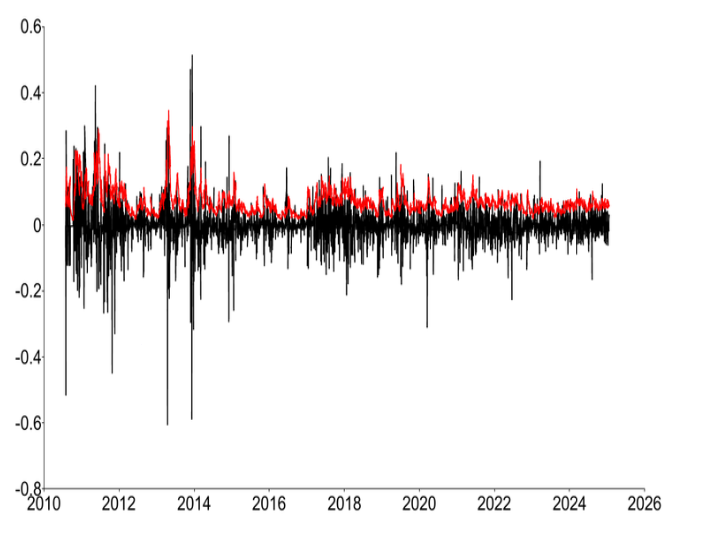
\includegraphics[
            width=0.50\linewidth
        ]{assets/bitcoin_volatility_comparison.png}

        \caption{Comparison of Beta-t-EGARCH
        and HF-Beta-t-EGARCH volatility
        estimates for Bitcoin.}

    \end{figure}

\end{block}


\begin{block}{Financial Assets Used}

    \begin{table}
        \centering

        \begin{tabular}{lccc}
            \toprule
            Asset & Ticker/Series & Absolute & RV \\
            \midrule
            Bitcoin & BITCOIN Index & 2.73 & 2.61 \\
            S\&P 500 & IVV US Equity & 2.18 & 2.25 \\
            Gold & IAU US Equity & 5.32 & 7.10 \\
            REIT & REIT Index & 3.16 & 2.93 \\
            Yen & FXY US Equity & 5.00 & 5.62 \\
            \bottomrule
        \end{tabular}

        \caption{Diebold--Mariano test
        statistics comparing Beta-t-EGARCH
        with HF-Beta-t-EGARCH.}

        \textbf{Data Source:} Bloomberg daily returns from July 19, 2010, to January 15, 2025.

        The dataset contains 3,648 observations per asset. Returns are demeaned before fitting.

    \end{table}

\end{block}

\begin{block}{Forecasting Methodology and Results}
      Out-of-Sample Forecasting Design

      \begin{itemize}
        \item \textbf{Forecasting approach:} One-day-ahead predictions using a rolling estimation window of 2,634 observations.
        \item \textbf{Forecast period:} January 4, 2021, to January 15, 2025, consisting of 1,014 observations.
        \item \textbf{Benchmark models:} Normal-GARCH, Beta-t-EGARCH, and HE-Beta-t-EGARCH.
        \item \textbf{Volatility proxies:} Absolute returns \(|y_t|\) and realized volatility (RV).
        \item \textbf{Evaluation methods:} Squared-error loss and Diebold–Mariano tests. Positive test statistics indicate superior forecasting performance for the HF model.
      \end{itemize}

    \begin{table}
        \centering

        \begin{tabular}{lccc}
            \toprule
            Asset & Ticker/Series & Absolute & RV \\
            \midrule
            Bitcoin & BITCOIN Index & 2.73 & 2.61 \\
            S\&P 500 & IVV US Equity & 2.18 & 2.25 \\
            Gold & IAU US Equity & 5.32 & 7.10 \\
            REIT & REIT Index & 3.16 & 2.93 \\
            Yen & FXY US Equity & 5.00 & 5.62 \\
            \bottomrule
        \end{tabular}

        \caption{Diebold--Mariano test
        statistics comparing Beta-t-EGARCH
        with HF-Beta-t-EGARCH.}

        \textbf{Data Source:} Bloomberg daily returns from July 19, 2010, to January 15, 2025.

        The dataset contains 3,648 observations per asset. Returns are demeaned before fitting.

    \end{table}

\end{block}

%------------------
% COLUMN #3
%-------------------

\end{column}

\separatorcolumn

% ==========================================
% COLUMN 3: RESULTS AND CONCLUSION
% ==========================================

\begin{column}{\colwidth}

% ==========================================
% SECTION 9: PREDICTIVE DENSITY COMPARISON
% ==========================================

\begin{block}{9. Predictive Density Comparison}

The Geweke--Amisano test statistics compare the
predictive density of HF-Beta-t-EGARCH against
each benchmark model.

Positive test statistics indicate superior
density forecasting performance for
HF-Beta-t-EGARCH.

\vspace{0.5cm}

\begin{table}
    \centering
    \small

    \resizebox{\linewidth}{!}{%
    \begin{tabular}{lccc}
        \toprule

        \textbf{Financial Asset}
        & \textbf{Normal-GARCH}
        & \textbf{Beta-t-EGARCH}
        & \textbf{HE-Beta-t-EGARCH} \\

        \midrule

        Bitcoin
        & $2.30^{**}$
        & $1.49$
        & $1.54$ \\

        S\&P 500 ETF
        & $1.71^{*}$
        & $1.56$
        & $1.45$ \\

        Gold ETF
        & $1.99^{**}$
        & $1.74^{*}$
        & $1.60$ \\

        S\&P US REIT
        & $2.78^{***}$
        & $2.75^{***}$
        & $2.39^{**}$ \\

        Japanese Yen Trust
        & $2.99^{***}$
        & $1.91^{*}$
        & $2.26^{**}$ \\

        \bottomrule
    \end{tabular}
    }

    \caption{
        Geweke--Amisano predictive density
        comparison test statistics.
    }

\end{table}

\vspace{0.3cm}

\footnotesize{
    $^{***}p < 0.01$,
    $^{**}p < 0.05$,
    $^{*}p < 0.10$.

    Source: Manuscript Table 2(c).
}

\vspace{0.5cm}

At the 10\% significance level,
HF-Beta-t-EGARCH demonstrates statistically
significant improvements over:

\begin{itemize}

    \item \textbf{Normal-GARCH:}
    Five out of five financial assets.

    \item \textbf{Beta-t-EGARCH:}
    Three out of five financial assets.

    \item \textbf{HE-Beta-t-EGARCH:}
    Two out of five financial assets.

\end{itemize}

\end{block}

% ==========================================
% SECTION 10: BITCOIN VOLATILITY PATHS
% ==========================================

\begin{block}{10. Illustration: Bitcoin Volatility Paths}

\textbf{Bitcoin Returns and Fitted Volatility,
2010--2025}

\vspace{0.5cm}

% Replace the file path below with the actual
% location of your Bitcoin comparison figure.
% If the image does not exist, a placeholder
% will appear instead of a compilation error.

\begin{figure}
    \centering

    \IfFileExists{assets/bitcoin_volatility_comparison.png}{%
        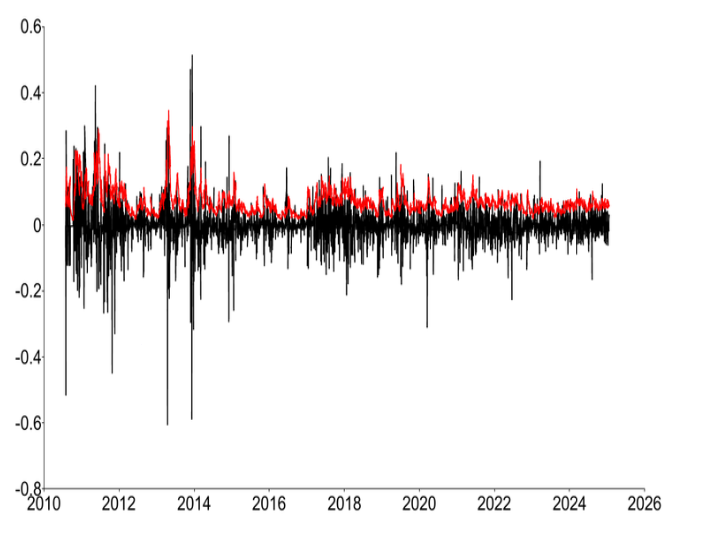
\includegraphics[
            width=0.95\linewidth
        ]{assets/bitcoin_volatility_comparison.png}
    }{%
        \fbox{%
            \parbox[c][5cm][c]{0.85\linewidth}{%
                \centering
                Insert Bitcoin volatility comparison figure
            }%
        }
    }

    \caption{
        Bitcoin daily returns and fitted volatility
        under Beta-t-EGARCH and HF-Beta-t-EGARCH.
        Source: Supplementary Figure A1(e)--(f).
    }

\end{figure}

\vspace{0.3cm}

Supplementary Figure A1(e)--(f) illustrates
daily Bitcoin returns (black) and fitted
volatility (red) from 2010 to 2025.

\begin{itemize}

    \item \textbf{Left Panel:}
    Beta-t-EGARCH.

    \item \textbf{Right Panel:}
    HF-Beta-t-EGARCH.

\end{itemize}

\end{block}

% ==========================================
% SECTION 11: INTERPRETATION AND IMPLICATIONS
% ==========================================

\begin{block}{11. Interpretation and Implications}

\textbf{Volatility Forecasting}

HF-Beta-t-EGARCH consistently improves
one-step-ahead volatility forecast performance
in this five-asset study.

\vspace{0.5cm}

\textbf{Density Forecasting}

Improvements relative to normal-GARCH are
widespread. However, statistical evidence of
improvements relative to other Beta-t-EGARCH
variants is less uniform.

\vspace{0.5cm}

\textbf{Practical Applications}

The findings suggest potential improvements
in financial risk forecasting and the
simulation of financial returns.

\end{block}

% ==========================================
% SECTION 12: SELECTED REFERENCES AND NOTES
% ==========================================

\begin{block}{12. Selected References and Notes}

\footnotesize{

\begin{enumerate}

    \item
    Blazsek, S., Escribano, A., \& Ayala, A.
    (2025).
    \textit{Improved Gradient Scaling for
    Score-Driven Filters with an Application
    to Stock Market Volatility.}

    \item
    Harvey, A. C., \& Chakravarty, T.
    (2008).
    \textit{Beta-t-(E)GARCH.}

    \item
    Bollerslev, T. (1986).
    \textit{Generalized Autoregressive
    Conditional Heteroskedasticity.}

\end{enumerate}

\vspace{0.3cm}

\textbf{Research Data and Results:}

Blazsek, Johnson, and Kobor.
\textit{An Empirical Application of Improved
Gradient Scaling for Score-Driven Volatility
Filters.}

Manuscript and supplementary material.

}

\end{block}

% ==========================================
% END OF COLUMN 3
% ==========================================

\end{column}


\separatorcolumn
\end{columns}
\end{frame}

\end{document}
